\documentclass{book}

\usepackage{listings}
\usepackage{theorem}
\usepackage{graphicx}
\usepackage{hyperref}
\usepackage{amsfonts}
\usepackage{amsmath}
\usepackage[table]{xcolor}
\usepackage{array,calc}
\usepackage{amsmath}

\newtheorem{exercise}{Exercise}


\lstset{
  language=Java,
  basicstyle=\ttfamily\footnotesize,
  numbers = left
}

\newcommand{\co}[1]{\lstinline[language=Java, basicstyle=\ttfamily]{#1}}

\begin{document}

\chapter{ImageJ}
ImageJ is a Java library for digital image analysis and processing. The library contains interfaces and classes for creating, modifying and displaying images. In this chapter, we explain how to perform basic image operations using this library.

\section{Setting up ImageJ}
ImageJ is a library for \emph{Java}. In the remainder of this section, we assume that a Java Development Kit (version 6 or higher) is installed on your machine. If Java is not installed on your machine, download and install a Java Development Kit from \href{http://www.oracle.com/technetwork/java/javase/downloads/index.html}{http://www.oracle.com/technetwork/java/javase/downloads/index.html}.

The ImageJ implementation, tutorials and additional documentation are available online at \href{http://rsbweb.nih.gov/ij}{http://rsbweb.nih.gov/ij}. To install ImageJ, download the platform independent release from \href{http://rsbweb.nih.gov/ij/download.html}{http://rsbweb.nih.gov/ij/download.html}. Extract the zip file to a location of your choice.

ImageJ can be used both as a standalone application and as a library. To run the application,  execute ImageJ.exe (on Windows) or ImageJ.app (on Mac). After starting the application, the following graphical user interface should be displayed on your screen:

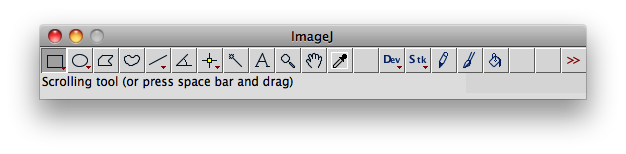
\includegraphics[scale=0.5]{ImageJ-screenshot.png}

\begin{exercise}
Perform edge detection using the ImageJ graphical user interface.
\begin{enumerate}
  \item Open an image via \texttt{File>Open...}.
  \item Detect edges in the image via \texttt{Process>Find Edges}.
\end{enumerate} 
Later in this course, we will explain how edge detection works and how it can be used to sharpen images and to perform seam carving.
\end{exercise}

The ImageJ library is packaged as a jar file called \texttt{ij.jar}. This jar file is located in the ImageJ directory. To use the interfaces and classes provided by ImageJ, \texttt{ij.jar} must be included in the classpath when compiling and running any program that uses the library.

\section{Images}
An image is a rectangular, two-dimensional grid of pixels, where each pixel represents the color at that location.



The most important classes for dealing with images in ImageJ is the class ImagePlus. This class contains method for accessing the with and height of an image. 

\begin{exercise}
Write a program that prints the width and height of an image. 
\end{exercise}

\section{Displaying an Image}

\section{Creating new images}

\section{Updating an image}

\section{Getting user input}

To modify an image, you have to use an ImageProcessor. 

\section{ImageJ Plugins}

\end{document}